% \documentclass[]{article}
\documentclass[12pt,titlepage,]{article}
\usepackage[T1]{fontenc}
\usepackage{lmodern}
\usepackage{amssymb,amsmath}
\usepackage{ifxetex,ifluatex}
\usepackage[left=2.6cm,top=3cm,right=2.6cm]{geometry}
\usepackage{fixltx2e} % provides \textsubscript
\usepackage[spanish]{babel}

% \renewcommand{\familydefault}{\sfdefault}

% use microtype if available
\IfFileExists{microtype.sty}{\usepackage{microtype}}{}
\ifnum 0\ifxetex 1\fi\ifluatex 1\fi=0 % if pdftex
  \usepackage[utf8]{inputenc}
\else % if luatex or xelatex
  \usepackage{fontspec}
  \ifxetex
    \usepackage{xltxtra,xunicode}
  \fi
  \defaultfontfeatures{Mapping=tex-text,Scale=MatchLowercase}
  \newcommand{\euro}{€}
\fi
\usepackage{color}
\usepackage{fancyvrb}
\DefineShortVerb[commandchars=\\\{\}]{\|}
\DefineVerbatimEnvironment{Highlighting}{Verbatim}{commandchars=\\\{\}}
% Add ',fontsize=\small' for more characters per line
\newenvironment{Shaded}{}{}
\newcommand{\KeywordTok}[1]{\textcolor[rgb]{0.00,0.44,0.13}{\textbf{{#1}}}}
\newcommand{\DataTypeTok}[1]{\textcolor[rgb]{0.56,0.13,0.00}{{#1}}}
\newcommand{\DecValTok}[1]{\textcolor[rgb]{0.25,0.63,0.44}{{#1}}}
\newcommand{\BaseNTok}[1]{\textcolor[rgb]{0.25,0.63,0.44}{{#1}}}
\newcommand{\FloatTok}[1]{\textcolor[rgb]{0.25,0.63,0.44}{{#1}}}
\newcommand{\CharTok}[1]{\textcolor[rgb]{0.25,0.44,0.63}{{#1}}}
\newcommand{\StringTok}[1]{\textcolor[rgb]{0.25,0.44,0.63}{{#1}}}
\newcommand{\CommentTok}[1]{\textcolor[rgb]{0.38,0.63,0.69}{\textit{{#1}}}}
\newcommand{\OtherTok}[1]{\textcolor[rgb]{0.00,0.44,0.13}{{#1}}}
\newcommand{\AlertTok}[1]{\textcolor[rgb]{1.00,0.00,0.00}{\textbf{{#1}}}}
\newcommand{\FunctionTok}[1]{\textcolor[rgb]{0.02,0.16,0.49}{{#1}}}
\newcommand{\RegionMarkerTok}[1]{{#1}}
\newcommand{\ErrorTok}[1]{\textcolor[rgb]{1.00,0.00,0.00}{\textbf{{#1}}}}
\newcommand{\NormalTok}[1]{{#1}}
% Redefine labelwidth for lists; otherwise, the enumerate package will cause
% markers to extend beyond the left margin.
\makeatletter\AtBeginDocument{%
  \renewcommand{\@listi}
    {\setlength{\labelwidth}{4em}}
}\makeatother
\usepackage{enumerate}
\usepackage{graphicx}
% We will generate all images so they have a width \maxwidth. This means
% that they will get their normal width if they fit onto the page, but
% are scaled down if they would overflow the margins.
\makeatletter
\def\maxwidth{\ifdim\Gin@nat@width>\linewidth\linewidth
\else\Gin@nat@width\fi}
\makeatother
\let\Oldincludegraphics\includegraphics
\renewcommand{\includegraphics}[1]{\Oldincludegraphics[width=\maxwidth]{#1}}
\ifxetex
  \usepackage[setpagesize=false, % page size defined by xetex
              unicode=false, % unicode breaks when used with xetex
              xetex]{hyperref}
\else
  \usepackage[unicode=true]{hyperref}
\fi
\hypersetup{breaklinks=true,
            bookmarks=true,
            pdfauthor={Borrador — Universidad Técnica Federico Santa María},
            pdftitle={Switch IDE},
            colorlinks=true,
            urlcolor=blue,
            linkcolor=magenta,
            pdfborder={0 0 0}}
\setlength{\parindent}{0pt}
\setlength{\parskip}{6pt plus 2pt minus 1pt}
\setlength{\emergencystretch}{3em}  % prevent overfull lines

\title{Switch IDE}
\author{\textbf{Borrador} --- Universidad Técnica Federico Santa María}
\date{Ian Murray Schlegel}

\begin{document}
\maketitle

% {
% \hypersetup{linkcolor=black}
% \tableofcontents
% }
 \pagenumbering{Roman}

\begin{flushright}
\topskip0pt
\vspace*{\fill}

\textit{A todos los que hicieron esto posible.}

\vspace*{\fill}
\end{flushright}

\newpage
\hypersetup{linkcolor=black} \tableofcontents

\newpage

\section{Introducción}

\pagenumbering{arabic}

En el contexto del desarrollo de aplicaciones web, existen dos grandes
``corrientes''. Por un lado, es posible (y se utiliza muchísimo)
desarrollar aplicaciones completamente de lado de servidor. Esto
significa que la aplicación procesa todos los datos y genera todo lo que
el usuario ve en el servidor. Esta forma de desarrollar ha sido así
durante muchísimos años y sigue siendo una forma muy utilizada. Por otro
lado, últimamente, con el crecimiento de la comunidad de Javascript, y
la constante mejora en rendimiento de los navegadores modernos, se ha
popularizado la idea de llevar gran parte de la lógica de negocio y el
procesamiento de datos al cliente. Los navegadores modernos tienen cada
vez más capacidad de ejecutar procesos rápida y eficientemente, lo que
tiene muchísimas ventajas: se aliviana la carga en los servidores, lo
que permite poder soportar a muchos más usuarios simultáneos; las
aplicaciones se desempeñan mucho mejor, dado que se disminuye el retardo
que hay en transmitir datos entre el cliente y el servidor. Esto último
es muy importante al momento de crear aplicaciones web. Si bien toda
página web, sin importar su naturaleza, debería ser lo más rápida y
responsiva posible, las aplicaciones web deben serlo por sobre todo. Al
fin y al cabo, están intentando imitar el comportamiento de aplicaciones
nativas, pero a su vez alivianando la carga a la que se somete un
desarrollador al momento de crear aplicaciones compatibles con una
infinidad de dispositivos y sistemas operativos distintos.

Desarrollar aplicaciones web versus desarrollar aplicaciones nativas
(que son ejecutables directamente en el computador, sin necesidad de un
navegador) tiene varias ventajas, siendo quizás la más importante que no
es necesario escribir el programa para diferentes plataformas, dado que
la mayoría de los navegadores modernos funcionan en una gran variedad de
dispositivos. Además, con el crecimiento del estándar HTML5 (que al
momento de escribir el presente documento aun se encuentra en proceso de
convertirse en un estándar final), es posible aprovechar muchas
características de los dispositivos (en algunos casos incluso es posible
usar los acelerómetros de los teléfonos móviles inteligentes). Es más,
muchos juegos han sido portados a la web, utilizando WebGL y tecnologías
similares.

Ahora bien, desarrollar aplicaciones web también tiene sus desventajas.
Es cosa de ver Xcode o Visual Studio, donde ambas herramientas son un
entorno completamente integrado para desarrollar aplicaciones. Desde
escribir código a crear formularios y diferentes tipos de vistas, ambas
herramientas y herramientas similares entregan una experiencia casi
inigualable al desarrollador. Al desarrollar aplicaciones y sitios web
en general, no es posible encontrar herramientas que se asemejen lo
suficiente a las mencionadas (y que sean de código abierto) como para
considerarse una alternativa viable. La mayoría de los entornos de
desarrollo para web permiten previsualizar lo que el desarrollador
codifica, pero no le permiten ahorrar tiempo al momento de realizar
tareas tan necesarias como codificar la interfaz de una aplicación.

Es este último aspecto el que se considera como un problema actualmente
en el mundo del desarrollo web. Si bien no es difícil codificar
interfaces de usuario al momento de crear aplicaciones web, es una tarea
que consume mucho tiempo y para la cual si existen herramientas muy
buenas en el mundo del desarrollo de aplicaciones nativas (como Xcode o
Visual Studio). Es por esto que en este trabajo se propone la creación
de un entorno de desarrollo integrado que permita la creación de
aplicaciones web facilitando la creación de interfaces de manera similar
a como lo hacen las herramientas ya mencionadas.

Este trabajo se estructurará como sigue:

\begin{itemize}
\item
  Se revisará primero el \emph{estado del arte}, analizando las
  herramientas que actualmente intentan dar solución al problema
  identificado, además de frameworks y otro tipo de utilidades que
  mitigan de cierta forma el problema pero sin darle una completa
  solución.
\item
  Luego se propondrá una solución al problema identificado, junto con
  métricas que permitirán cuantificar la efectividad de la solución
  creada.
\item
  Se construirá y documentará la creación de la solución planteada,
  comentando en el proceso la efectividad de las herramientas escogidas.
\item
  \textbf{NO SE AUN} Se mostrarán casos de uso de la aplicación creada
  de manera de mostrar su funcionamiento
\item
  Se analizarán los resultados utiliando las métricas previamente
  propuestas.
\item
  Finalmente se presentarán conclusiones del trabajo junto con ideas
  para posible trabajo futuro.
\end{itemize}

\newpage

\section{Estado del Arte}

La metodología para el desarrollo de aplicaciones web está cambiando. Ha
pasado de estar enfocada casi completamente de desarrollar de lado de
servidor a desarrollar parcial o totalmente de lado de cliente.
Frameworks como Backbone han revolucionado lo que se piensa sobre
desarrollar aplicaciones completamente usando Javascript, y la aparición
de muchísimos frameworks nuevos en este joven sub-mundo de aplicaciones
muestra claramente una tendencia hacia este ``paradigma''.

Ahora bien, el hecho de que periódicamente aparezcan nuevos frameworks
no es necesariamente bueno. Es fácil perderse, no se puede saber por
dónde empezar, y lo peor de todo, cada framework hace lo suyo de formas
diferentes, incluso utilizando paradigmas de desarrollo distintos (ya
sea MVC {[}1{]}, MVP {[}2{]} u otro de los que normalmente se utilizan).

En este capítulo, se revisarán las diferentes herramientas que existen
el mundo del desarrollo de aplicaciones Javascript, además de programas
y utilidades que funcionan de manera similar a lo que se quiere lograr
con Switch IDE y que están actualmente en el mercado. Se revisarán
primero diferentes frameworks disponibles hoy en día, analizando sus
ventajas y desventajas, para luego mostrar herramientas que facilitan el
uso de frameworks y otro tipo de soluciones online.

\subsection{Frameworks Actuales}

Existe una variedad enorme de frameworks para desarrollo web de lado de
cliente, y, como se dijo anteriormente, día a día aparecen nuevos
competidores, lo que pasó de ser algo bueno a algo que aumenta las
barreras de entrada. El hecho de que haya tantas opciones para
desarrolladores (incluso experimentados) hace que elegir uno sea muy
difícil y que finalmente se opte por la solución incorrecta. Muchos
frameworks tienen varios puntos fuertes, y no siempre un framework es la
mejor solución para un tipo determinado de problema.

Ahora bien, sí existen buenos frameworks y varios de ellos son
relativamente fáciles de entender y dominar. La mayoría de ellos llevan
buen tiempo en el mercado y por ende tienen una comunidad fuerte y
activa, junto con una base de código robusta.

\subsubsection{Backbone}

\href{http://backbonejs.org}{Backbone} {[}3{]} es uno de los frameworks
más populares. Basta con ver la gran cantidad de sitios que lo utilizan
actualmente {[}4{]}. Es simple, extensible y muy poderoso, lo que lo
hace una muy buena opción para desarrollar aplicaciones responsivas.
Además, sus pocas dependencias hacen que las aplicaciones desarrolladas
con él sean livianas.

El objetivo principal de Backbone es facilitar y dar estructura a
aplicaciones que se basan fuertemente en funcionar del lado del cliente
(es decir, en el navegador mismo). Normalmente, escribir aplicaciones de
este estilo es posible utilizando sólo Javascript y sin usar algún
framework, pero ello resulta tedioso, y lleva a aplicaciones difíciles
de mantener. Backbone (y la mayoría de los frameworks que se nombrarán
en este capítulo) intentan evitar esto último dándole una estructura a
las aplicaciones, separando vistas de controladores y modelos, y dejando
las cosas en su lugar. Trae consigo facilidades para guardar información
en servidores (en cierta forma proveyendo un ``backend'' a las
aplicaciones que se creen). Además, facilitan la interacción con el
usuario, a la larga ahorrando tiempo al desarrollador.

Es utilizado por un sinfín de proyectos, algunos muy populares, tales
como \href{http://www.groupon.com/now}{Groupon Now!},
\href{http://trello.com}{Trello}, entre otros {[}4{]}. Las aplicaciones
nombradas no son proyectos pequeños y simples, sino que son aplicaciones
muy poderosas que se benfician muy bien de lo que Backbone provee.

\subsubsection{Cappuccino}

\href{http://cappuccino-project.org}{Cappuccino} {[}5{]} es un framework
de desarrollo web enfocado en llevar ``Cocoa'' de Apple a la web, aunque
no está en forma alguna afiliado con esta empresa. Abstrae completamente
el desarrollo web a un único lenguaje: Objective-J, un superconjunto de
Javascript (de la misma forma que Objective-C es un superconjunto de C).
No cuenta con demasiados adeptos, dado que no muchos sitios lo utilizan,
pero el framework sigue en constante desarrollo, aunque con una
comunidad menor que la de Backbone, eso sí.

Las ventajas de este framework son varias. Al estar imitando bastante
fuertemente a Apple, sigue varios estándares ya conocidos, y lo hace
bastante fácil de aprender para una persona con experiencia en
desarrollo iOS o Mac OS X. Además, todo se desarrolla con el mismo
lenguaje, y trae integrados varios controles (botones, tablas, ventanas,
menús), lo que le permite al desarrollador enfocarse sólo en código y no
en el diseño (ver Figura \ref{figure:cappuccino}). A diferencia de
Backbone, en donde el desarrollador debe trabajar por un lado con el
código y por otro con el diseño y los estilos de las aplicaciones,
Cappuccino trae todo eso en un solo framework, de la misma forma que
Visual C\# trae sus controles y el diseño incorporados, por ejemplo.

\begin{figure}[htbp]
\centering
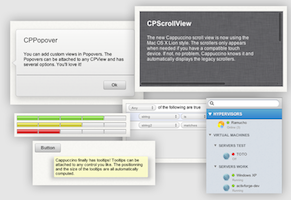
\includegraphics{figures/cappuccino-widgets.png}
\caption{Un ejemplo de los diferentes controles que vienen incluidos en
Cappuccino. Puede apreciarse el diseño estilo OS X que trae.
\label{figure:cappuccino}}
\end{figure}

Una de las características interesantes de este framework (aunque no es
la que más se publicita), es la capacidad de usar el constructor de
interfaces de \href{https://developer.apple.com/xcode/}{Xcode} {[}6{]}
--- Interface Builder --- para crear las interfaces. Eso sí, no todos
los componentes que están disponibles en Xcode están implementados en
Cappuccino, y agregar elementos inexistentes no siempre arroja errores
fáciles de descubrir. Además, desarrollar usando esta técnica, requiere
instalar varios componentes (entre ellos, Xcode, que no es liviano) y se
necesita un computador Mac, dado que Xcode no funciona en otras
plataformas. Por si eso no fuera poco, el ir y venir entre Xcode y el
editor que se use para Cappuccino hace que la experiencia sea todo menos
placentera para el desarrollador.

Además de lo anterior, tiene otras desventajas. Por un lado, es
necesario aprender un lenguaje nuevo (Objective-J) y utilizar un
framework completamente distinto a todos los conocidos (casi todos están
programados en Javascript directamente). Por otro lado, hay varios
controles esenciales que no están implementados, como por ejemplo, un
control de entrada de texto multilínea no está soportado actualmente por
el framework (aunque existen herramientas de terceros).

\subsubsection{Ext JS}

\href{http://www.sencha.com/products/extjs/}{Ext JS} {[}7{]} es un
framework con bastante tiempo en el mercado. Tiene soporte para una gran
variedad de componentes y es muy poderoso. Una de las ventajas
importantes de este framework, es que existe una empresa bastante
importante detrás: \href{http://www.sencha.com/}{Sencha Inc}. Esto
asegura que el framework tiene soporte detrás, y que existe mucha gente
preocupada constantemente de su desarrollo. Incluso, esta empresa ofrece
soporte técnico pagado para este framework.

Este es un framework bastante poderoso, a la par e incluso por sobre
Cappucino y otros similares. Al llevar bastante tiempo circulando (desde
el 2007 {[}8{]}), es un framework con una gran cantidad de componentes y
características disponibles que lo hacen muy poderoso. Se diferencia en
casi las mismas cosas con Backbone que Cappuccino, al tener integrados
muchísimos componentes como botones, tablas, ventanas, entre otros, pero
con la diferencia de que este framework sí está escrito en Javascript
directamente, por lo que no hace falta aprender un lenguaje nuevo.

Ahora bien, tiene sus desventajas. Es un framework muy completo y
dominarlo toma más tiempo que otros. No es un framework fácil de usar y
no existe una gran comunidad detrás (no existen muchos sitios
desarrollados con esta plataforma, al menos no sitios públicos), por lo
que encontrar tutoriales e información al respecto no es tarea fácil.
Además, una de las mayores desventajas, es que este framework no es
gratuito para desarrollo comercial. Si se desea desarrollar una
aplicación web y mantener el código propietario, se deben cancelar (por
lo bajo) \$329 dólares americanos {[}9{]}, valor a veces prohibitivo
considerando que la mayoría de los otros frameworks son gratuitos.

\subsection{Herramientas Actuales}

Ahora que se han visto una variedad de frameworks disponibles para
desarrollar aplicaciones web, se procederá a analizar el mundo de las
herramientas para el desarrollo de éstas. El enfoque de esta sección es
analizar diferentes programas y servicios que se ofrecen, que son en
alguna forma similares a lo que se quiere lograr con Switch IDE.

\subsubsection{Sencha Architect}

Si se tuviera que elegir una herramienta para describir lo que se quiere
lograr con Switch, sería
\href{http://www.sencha.com/products/architect}{Sencha Architect}
{[}10{]}. Sencha Architect es una herramienta de los mismos creadores
del framework Ext JS, y es lo que más se asemeja a lo que se quiere
lograr con esta memoria. Es bastante poderosa, y permite desarrollar
aplicaciones web y móviles (basadas en web, no nativas) de manera
visual, de una forma bastante similar a lo que se quiere lograr con
Switch IDE.

\begin{figure}[htbp]
\centering
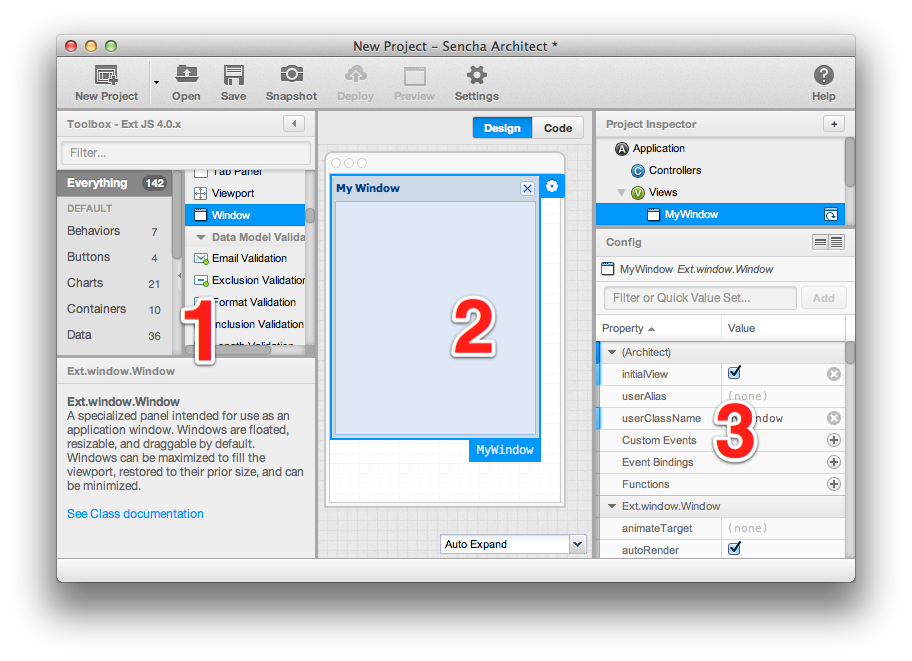
\includegraphics{figures/sencha-architect-big.png}
\caption{Sencha Architect: La ventana de trabajo
\label{figure:sencha-architect}}
\end{figure}

Sencha Architect es la herramienta que más se asemeja a un IDE para
desarrollo de aplicaciones nativas (como Xcode o Microsoft Visual
Studio). Posee una barra lateral con componentes (ver Figura
\ref{figure:sencha-architect}, el número 1), un área central de trabajo
(número 2) y propiedades de los diferentes componentes que existan en el
área de trabajo (número 3).

Las ventajas de esta herramienta son claras: es posible crear las vistas
de las aplicaciones directamente, arrastrando componentes. De la misma
forma que herramientas para desarrollo nativo, esto ahorra tiempo al
momento de desarrollar.

Las desventajas son varias, eso sí. Por un lado, el desarrollador está
obligado a trabajar con Ext JS como framework (que, como ya se dijo
antes, no es fácil de aprender y usar), y por otro lado, la licencia de
uso de este software no deja de ser considerable: \$399 dólares
americanos {[}11{]} al momento de escribir este documento. Esto es un
monto realmente alto, pues si se compara esto con el precio de un editor
de código relativamente bueno (como lo son TextMate o Sublime Text 2,
ambos cercanos a los \$50 dólares), es una inversión de consideración.
Además, a ese valor hay que agregarle otros \$329 por la licencia de uso
de Ext JS {[}9{]}, si es que se quiere para uso comercial.

\subsubsection{Divshot}

\href{http://divshot.com/}{Divshot} {[}12{]} es una de las herramientas
que inspiró la presente memoria. Es una aplicación de prototipado rápido
basado en web. Fue creada en abril de 2012, por lo que es una
herramienta relativamente nueva y, de hecho, no está abierta al público
aún. Se logró conseguir una licencia de uso en esta fase para poder
estudiar el poder de esta herramienta, y se llegó a la conclusión de que
realmente tiene mucho potencial.

Permite, utilizando Twitter Bootstrap {[}13{]}, crear prototipos de
sitios y aplicaciones web arrastrando componentes, de la misma forma que
IDEs como Xcode o Microsoft Visual Studio. En la presente memoria, se
quiere lograr un comportamiento muy parecido para la creación de vistas,
por lo que se podría considerar que Divshot es una de las inspiraciones
más grandes para esta memoria.

Entre las ventajas que presenta la herramienta, está la facilidad con la
que se pueden crear prototipos de vistas. Sólo arrastrando componentes,
se puede llegar a una vista en pocos minutos. Además, es posible
previsualizar los resultados fácilmente, e incluso exportar a
HTML\footnote{\textbf{Hypertext Markup Language:} es el lenguaje de
  etiquetas utilizado para las páginas web. Todas ellas están hechas con
  esto, más una combinación de otros lenguajes. {[}14{]}} con un sólo
click. Lo mejor de todo, es que el HTML generado está muy bien ordenado
y formateado.

Desventajas no tiene muchas. Es una herramienta muy puntual y bien
diseñada, y, como aún está en fases de desarrollo, en constante mejora.
Ahora bien, no es un ``competidor'' directo de Switch IDE, dado que no
es una herramienta para programar. Simplemente permite crear vistas, que
es sólo un componente de Switch.

\begin{figure}[htbp]
\centering
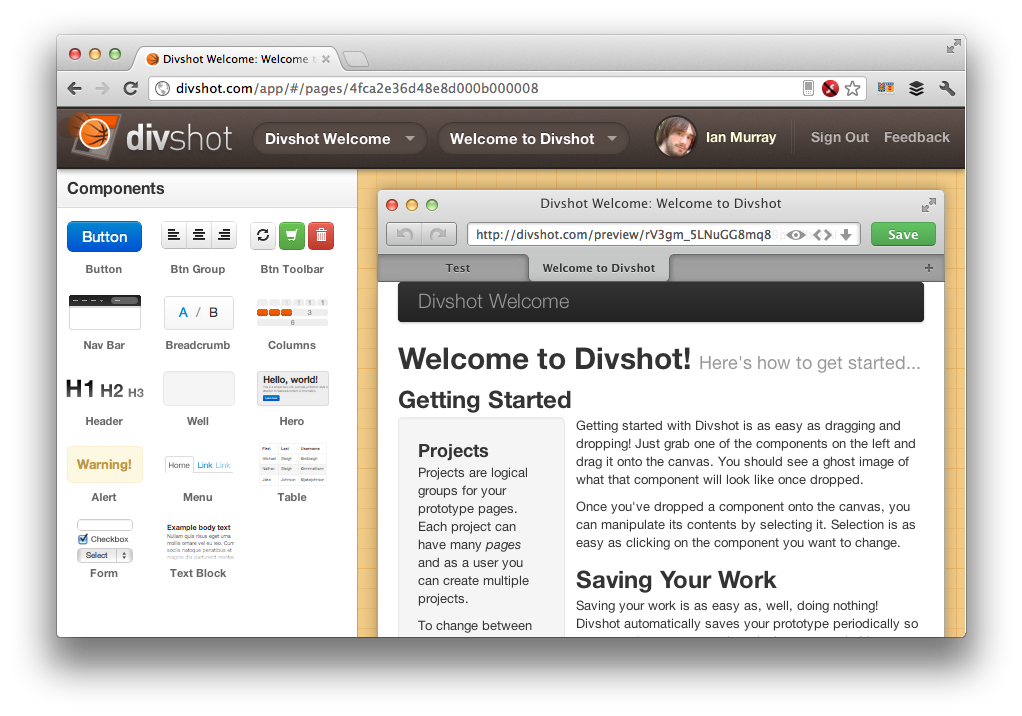
\includegraphics{figures/divshot-big.png}
\caption{La ventana principal de Divshot. Se pueden apreciar los
componentes en la barra lateral izquierda, con la vista a la derecha,
donde se arrojan los componentes. \label{figures:divshot}}
\end{figure}

\subsubsection{eXo Cloud IDE}

\href{http://cloud-ide.com}{eXo Cloud IDE} {[}15{]} es un entorno de
desarrollo integrado, en la nube. Tiene varias características que lo
hacen una buena opción al momento de querer colaborar o mantener el
código alojado en internet. Soporta una gran variedad de lenguajes
(entre ellos Java, Ruby y Python) y frameworks (como Ruby on Rails,
Spring o incluso Google App Engine).

Además de lo anterior, soporta plataformas como Heroku para subir
cambios a servidores directo desde el navegador, e incluso tiene soporte
para versionamiento con Git {[}16{]}.

Como cualquier IDE nativa estilo Xcode o Microsoft Visual Studio, tiene
un visor de los archivos actualmente abiertos (ver Figura
\ref{figure:exo-ide}, número 1) y el editor de código mismo (número 2).

\begin{figure}[htbp]
\centering
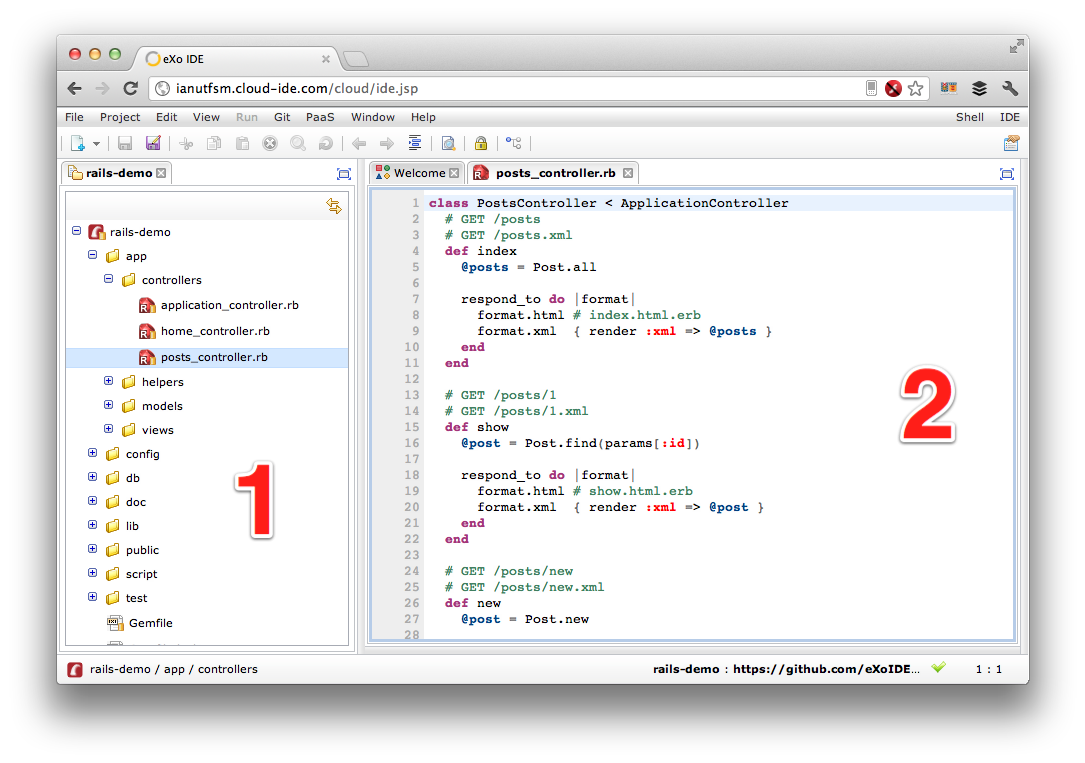
\includegraphics{figures/exo-ide-big.png}
\caption{eXo Cloud IDE: un entorno de desarrollo integrado, en la
nube\label{figure:exo-ide}}
\end{figure}

Las ventajas que provee esta herramienta son el no tener que depender de
un sólo equipo para desarrollar. Al mantener el código en la nube, sólo
es necesario conectarse al sitio web y empezar a trabajar. Por esto
último, tampoco es necesario instalar las diferentes herramientas
necesarias para desarrollar (como puede ser instalar Ruby o Python, que
a veces es engorroso).

Ahora bien, tiene sus desventajas, siendo la más importante el hecho de
que no permite desarrollar vistas de forma visual (que es lo que uno
espera de una herramienta integrada de este estilo). Además, al no estar
enfocado en un framework de desarrollo específico, no es muy poderoso al
momento de elegir alguno (en términos de autocompletado de código por
ejemplo). Relacionado con esto último, no permite desarrollar
aplicaciones de lado de cliente, sólo de lado de servidor, por lo que
también está limitado por ese lado. Además, desarrollar aplicaciones con
los frameworks que soporta por lo general implica utilizar mucho el
terminal de comandos para realizar pruebas, y en un ambiente web, eso no
es fácilmente replicable.

\subsubsection{Wavemaker}

\href{http://www.wavemaker.com/}{Wavemaker} {[}17{]} es una herramienta
que permite generar ``bases de datos'' de manera visual. El objetivo
principal de esta aplicación es poder crear sistemas de manejo de datos
de manera fácil, escribiendo la menor cantidad de código posible.

Esta herramienta se asemeja más a lo que es Microsoft Access. La idea es
poder crear interfaces para guardar y organizar información rápidamente
y sin programar. Es una aplicación enfocada más a gente que no tiene
conocimientos de programación, aunque según los creadores de Wavemaker,
las aplicaciones que se generan son aplicaciones Java completas, que
pueden ser extendidas más adelante programando Java directamente.

Las ventajas dependen realmente de lo que se quiera hacer con la
herramienta. Si el usuario no tiene conocimientos en el área de
desarrollo de software, entonces la herramienta es bastante útil, aunque
los resultados no son muy complejos. Por otro lado, si se le mira desde
el punto de vista de un desarrollador, la herramienta no ofrece mayores
beneficios a las anteriormente mencionadas.

\subsubsection{Zoho Creator}

\href{http://www.zoho.com/creator/}{Zoho Creator} {[}18{]} es un
servicio web que tiene más o menos el mismo enfoque que Wavemaker: crear
bases de datos simples sin programar. Ahora bien, se diferencia un poco
con Wavemaker en el sentido de que es un servicio, pagado, que permite
crear aplicaciones en la nube y mantenerlas ahí, mientras que la
herramienta anterior permite crearlas y exportarlas, para luego incluso
extenderlas si es que se tienen conocimientos.

Si bien Zoho Creator es una herramienta relativamente poderosa y fácil
de usar, no es una herramienta que utilizaría un desarrollador. Hay
varias razones para esto último. Primero, no permite exportar lo creado
para alojarlo en otro servidor; segundo, no es una herramienta de
desarrollo que permita crear aplicaciones de lado de cliente o de
servidor, sino que permite crear simples bases de datos; y tercero, no
es una herramienta gratuita o de código abierto, lo que hace que lo
creado con ella tenga ciertas limitaciones en cuanto a licencias.

\newpage

\section{Propuesta de Solución}

Para solucionar el problema identificado, se propone una herramienta
web, basada en \emph{Backbone} y \emph{Ruby}, que permita editar una
aplicación web completa en el mismo navegador. Sus principales
características serían:

\begin{itemize}
\item
  Dar una estructura a las aplicaciones que se desarrollen con Backbone
\item
  Facilitar la creación de vistas mediante un editor que permita
  arrastrar los diferentes componentes y ahorrar el tiempo gastado en
  ello
\item
  Implementar atajos de teclado de manera similar a cómo lo haría una
  IDE de escritorio
\end{itemize}

La herramienta no puede funcionar sólo de lado de cliente
(exclusivamente en el navegador), dado que algunas funciones deben ser
ejecutadas en el servidor, como por ejemplo la compilación de los
archivos Javascript y levantar una instancia de un servidor para probar
lo que el usuario esté desarrollando. Por esto, es necesario implementar
este proyecto en dos partes distintas, pero dependientes.

Por un lado, se tiene el servidor, que tendrá la tarea de manipular los
archivos de cada proyecto que el usuario cree y desarrolle. Además,
tendrá la tarea de ejecutar ciertos comandos necesarios para la creación
y prueba de los proyectos, que simplemente no es posible ejecutar en el
navegador. El hecho de que exista un ``backend'' como se le llamará de
ahora en adelante, permite además dar lugar a futuras características
imposibles de llevar a cabo, como por ejemplo soporte para repositorios
Git, que deben ser manejados en el servidor exclusivamente.

Por otro lado, está el cliente. El cliente es básicamente el
``frontend'' (como se le llamará de ahora en adelante). Es la interfaz
gráfica y es lo que interactúa con el usuario, en el navegador. La mayor
parte del trabajo recaerá en esta parte, dado que es lo que el usuario
ve y utiliza para trabajar. Además, es la parte del proyecto que
contendrá el editor de vistas, lo que requerirá un esfuerzo no mínimo
para funcionar.

\subsection{Elección de Herramientas para el Backend}

Para desarrollar el backend se escogió el lenguaje de programación
\emph{Ruby}. Las razones para la elección de este lenguaje son varias:
la familiaridad que tiene el autor con éste; su simplicidad para
desarrollar tareas relativamente complejas en otros lenguajes; la
infinidad de librerías disponibles para facilitar diferentes tareas
(como por ejemplo \emph{Grit}, una librería para manejar repositorios
Git directo desde Ruby).

Para desarrollar el backend no se utilizará Ruby puro. Lo que se quiere
desarrollar en el lado del backend es básicamente una API (Application
Programming Interface), que el frontend utilizará parar funcionar
correctamente. Existen varias formas de programar APIs en Ruby, donde
las más populares son Ruby on Rails y Sinatra.

La primera --- Ruby on Rails --- ha comenzado a ser muy popular en estos
últimos años por ser un framework extremadamente completo. Facilita
enormemente una infinidad de tareas que lo hacen una herramienta ideal
para todo tipo de proyectos web. Sin embargo, al ser una herramienta tan
completa, agrega bastante \emph{overhead}. Además, es una herramienta
ideal para crear proyectos grandes y muy complejos, y dado que el
backend de el presente trabajo no requerirá tanta complejidad, se
convierte en una alternativa no tan ideal para este trabajo.

La segunda --- Sinatra --- podría considerarse el hermano menor de Ruby
on Rails. Es un framework muchísimo más simple, y, por ende, mucho más
liviano. Inicia más rápido y, en general, se desempeña mejor que su
contraparte. Tiene la desventaja de no poseer tantas facilidades para
desarrollar sitios complejos y grandes, pero dado que el backend de este
proyecto no requerirá tanto trabajo, es la opción ideal.

\subsection{Elección de Herramientas para el Frontend}

Dado que la solución que se propone es una herramienta para desarrollar
aplicaciones en Backbone utilizando Twitter Bootstrap, lo lógico es
desarrollar esta solución usando las mismas herramientas. Se escogió
Backbone dada su alta popularidad. Esto asegura que el framework es
bastante sólido y que existen variadas librerías y herramientas estables
para él. Por otro lado, si bien Backbone es un framework poderoso, es
bien simple, lo que da más libertad sobre como afrontar diferentes
problemas.

Ahora, Backbone es un framework que no da una estructura a las
aplicaciones que se desarrollan con él. A diferencia de Ruby on Rails,
por ejemplo, la tarea de estructurar la aplicacion en carpetas o módulos
depende completamente del desarrollador. En este punto se asemeja mucho
más a Sinatra que a Ruby on Rails. Esto puede considerarse una
desventaja, dado que sistemas complejos tienden a crecer y desordenarse
bastanta si no se aplica una estructura desde un principio. Por esto, es
que se decidió utilizar Brunch\footnote{Poner referencia a esto!}.
Brunch es un ensamblador de aplicaciones (``application assembler'' en
inglés). Básicamente, basándose en un esqueleto, organiza aplicaciones
en carpetas. Soporta diferentes frameworks y lenguajes, desde Backbone a
Knockout\footnote{Referencia!}, usando Javascript o
Coffeescript\footnote{Referencia.}. Además de entregar una estructura,
las ensambla, es decir, toma todos los archivos y los junta en uno sólo
de manera de optimizar la aplicación cuando esté en producción. Es más,
incluye un servidor web de desarrollo, que detecta cambios en los
archivos y reensambla todo el sitio de manera de poder hacer pruebas más
rápida y fácilmente.

En lo que respecta la decisión de lenguaje de programación, no hay
muchas alternativas. Es posible desarrollar la solución usando
Javascript o Coffeescript. Existen otras alternativas, pero al momento
de escribir este documento no se encuentran en etapas estables de
desarrollo ni madurez. Javascript es un lenguaje poderoso pero a la vez
de relativo bajo nivel. Ciertas cosas son un tanto tediosas de
programar, como recorrer arreglos por ejemplo. En cambio, Coffeescript,
un lenguaje de programación escrito por Jeremy Ashkenas que apareció en
el 2009\footnote{Https://github.com/jashkenas/coffee-script/commit/8e9d637985d2dc9b44922076ad54ffef7fa8e9c2.}
que compila a Javascript, hace que desarrollar en Javascript sea mucho
más cómodo y simple, sin perder desempeño ni funcionalidad (pues compila
directamente a Javascript). Además, hace muchísimo más fácil programar
``orientado a objetos''. Si bien ECMAScript (la base de Javascript) está
definido como orientado a objetos,\footnote{Http://www.ecma-international.org/publications/files/ECMA-ST/Ecma-262.pdf
  página 1.} su estilo es diferente al resto de los lenguajes.
Coffeescript agrega palabras clave como \texttt{class} y
\texttt{extends} de manera de facilitar escribir clases y manipular
objetos en este lenguaje.

Por último, para el diseño y estructura de la interfaz, se decidió
utilizar \emph{Twitter Bootstrap}. Bootstrap es un conjunto de
componentes y un sistema de estructurado para páginas web, que hace la
tarea de crear y diseñar un sitio muy simple. Trae consigo una enorme
cantidad de componentes (botones, barras de progreso, etc.), además de
facilitar el diseño de formularios y componentes similares muy comunes
al momento de crear aplicaciones web. No sólo se utilizará Twitter
Bootstrap para crear el frontend, sino que también se utilizará para el
diseñador de interfaces, dado que tiene todas las ventajas descritas
anteriormente.

\newpage

\section{Construcción de la Solución}

Este capítulo tiene por objetivo detallar todo el proceso del diseño y
desarrollo de la solución propuesta anteriormente. Se dividirá en los
siguiente subcapítulos:

\begin{enumerate}[a.]
\item
  Diseño de la solución: básicamente se explicará cómo ambas componentes
  (frontend y backend) interactuarán entre sí. Además, cómo funcionarán
  ambas partes en términos de manipulación de archivos y el proyecto
  completo. Por último, se explicará cómo se diseñó el componente
  principal de la solución (el editor de interfaces).
\item
  Flujo del usuario: \textbf{\emph{EXPLICAR ESTO, SON BÁSICAMENTE CASOS
  DE USO}}
\item
  Primera etapa de construcción: el desarrollo de la solución se dividió
  en dos etapas principalmente. Primero, se desarrolló lo que se
  denominó una ``base'' del programa. Esta etapa contempló el desarrollo
  de gran parte del backend y, en el frontend, una herramienta que
  permitiera crear proyectos nuevos, crear, editar y eliminar archivos,
  compilar y correr el proyecto.
\item
  Primera etapa de construcción: la segunda parte del desarrollo se
  enfocó en desarrollar y perfeccionar el editor de interfaces. Dado que
  este componente es el grueso de la solución, se decidió dedicar una
  etapa completa a él.
\end{enumerate}

\subsection{Diseño de la Solución}

\subsubsection{Backend}

La solución es una aplicación mayoritariamente de lado de cliente, por
lo que la mayor cantidad de lógica debe ir en este lado. Por esta razón,
se diseñó el servidor de la forma más simple posible. Las tareas
principales que tiene el servidor o backend de la aplicación son:

\begin{itemize}
\item
  Autentificar usuarios
\item
  Generar proyectos utilizando Brunch
\item
  Manipular los archivos. Esto incluye crear, eliminar, renombrar y
  actualizar archivos (o sea, recibir el contenido de ellos y guardarlo
  a disco)
\item
  Ensamblar el proyecto
\item
  Levantar un servidor estático que permita al usuario probar su
  proyecto
\end{itemize}

Algunas de estas tareas son realizadas por la utilidad Brunch, por lo
que sólo es necesario hacer que el servidor ejecute un comando en la
consola para llevarlas a cabo. El resto de las tareas son básicamente
manipulación de archivos, para lo cual cualquier lenguaje de
programación trae funciones o librerías (y Ruby no es ninguna
excepción).

Se decidió utilizar una aproximación a lo que es REST\footnote{Explicar
  esto.} para los servicios que proveerá el backend. En REST, la idea es
representar objetos, y exponer diferentes métodos para tales objetos. En
este caso, se decidió que deben existir 3 objetos diferentes: usuarios,
proyectos y archivos.

\begin{itemize}
\item
  Usuarios: dado que la idea es que varios usuarios puedan utilizar el
  sistema a la vez, debe existir esta entidad en el servidor (y por ende
  en la base de datos).
\item
  Proyectos: es casi la base de todo. Cada proyecto contendrá los
  diferentes archivos y carpetas, y pertenecerá a un usuario.
\item
  Archivos: esto se refiere a archivos y carpetas. Por la forma en la
  que se manipulan los archivos en el servidor y en el cliente, es más
  conveniente manejarlos de (casi) la misma forma. Esto último se
  refiere a la forma en la que se obtienen los archivos en el servidor,
  y las acciones que se realizan en ellos. Ambos archivos y carpetas se
  crean y eliminan, como también se renombran. La única diferencia
  substancial es que las carpetas no tienen contenido y no se actualizan
  como el resto de los archivos.
\end{itemize}

El servidor autentificará a los usuarios utilizando sus cuentas de
GitHub y OAuth. OAuth es un protocolo de autentificación y autorización
que permite al usuario registrarse e ingresar a la aplicación con un
sólo click (dos si ingresa por primera vez). Dado que esta es una
herramienta enfocada a programadores, y considerando que GitHub es una
plataforma conocida por cualquier desarrollador que se mantenga al día,
utilizar este sistema para autentificar a los usuarios es simple y
conveniente. Por el lado de servidor, basta con incluir una librería que
redirige a los usuarios a las URLs específicas y crear un registro en la
base de datos si es que el usuario está ingresando por primera vez.

\subsubsection{Frontend}

El frontend tendrá dos tareas principalmente. Primero, deberá permitir a
los usuarios autentificarse. Para esto, y para efectos del presente
trabajo, será una simple página web que redirija al usuario a GitHub
para autentificarse usando este sistema. Segundo, deberá proveer al
usuario con la IDE que se quiere construir en este documento.

\textbf{\emph{EXPLICAR DE QUÉ TRATA LA PÁGINA DE AUTENTIFICACIÓN A
GRANDES RASGOS, SCREENSHOTS Y TODO}}

La IDE misma se dividirá en tres componentes principales: la barra
lateral izquierda para explorar los archivos del proyecto, la barra
lateral derecha con componentes visuales (como botones, formularios,
etc.), y la sección central que contendrá el código del archivo
actualmente seleccionado o la vista previa en caso de estar editando una
vista.

Contará además con una barra superior con un menú (al igual que
cualquier aplicación de escritorio), pero dado que proveerá simples
accesos directos a funciones que se explicarán más adelante no se
detallará su diseño ni implementación.

En los siguientes párrafos se pretende explicar qué objetos existirán en
el frontend, sus responsabilidades y cómo interactuarán entre ellos.
Primero se definirán algunos conceptos necesarios para entender de qué
tipos de objetos se estará hablando.

\textbf{Modelo:} Representa un objeto en un proyecto, como por ejemplo
un archivo, una carpeta o el proyecto mismo. Cada modelo es responsable
de persistir su estado de alguna forma (comunicándose con un servidor o
almacenando datos en el mismo navegador).

\textbf{Colección:} Es básicamente una lista de instancias de un tipo de
modelo. Por ejemplo, una carpeta podría considerarse una colección de
archivos (siendo cada archivo una instancia de un modelo).

\textbf{Vista:} Una vista en Backbone es un archivo que se encarga de
presentar información al usuario, y además de interactuar con él, por
ejemplo ejecutando funciones cuando se haga un click en un botón. Una
vista por lo general presenta un modelo (o una colección). Por ejemplo,
se puede tener una vista para cada instancia de un archivo, o bien se
pueden tener vistas que no presenten a ningún modelo en particular.

\textbf{Template:} Un template es un trozo de HTML que una vista utiliza
para generar lo que el usuario ve. Si bien no son enteramente necesarias
y una vista podría generar todo lo que necesita con Javascript, hacen la
tarea algo más fácil.

A continuación se explicará a grandes rasgos los modelos y colecciones
que existirán en el frontend. Se tendrán modelos para los proyectos y
los archivos. Cada uno se encargará de comunicarse con el backend para
obtener los datos que le sean necesarios o bien para guardar los
cambios.

\textbf{El modelo de proyecto} guardará el nombre de éste y una
referencia a una colección de los archivos que se encuentren en la raíz
de su carpeta. Tendrá como responsabilidades crear archivos y carpetas,
ensamblar el proyecto e iniciar el servidor de pruebas. Estas acciones
se complementan con llamadas al backend que realizan las tareas mismas.

\textbf{El modelo de archivo} se encargará de guardar el nombre y el
contenido (en caso de que corresponda) del archivo o carpeta al que
representa, además de guardar una referencia al proyecto al que
pertenece y . Tendrá como responabilidades pedir su contenido,
actualizarlo, renombrar y eliminar el archivo del sistema. Todas estas
acciones se complementan además con llamadas al backend.

\textbf{La colección de archivos} tendrá como responsabilidad ordenar
las listas de archivos una vez que la haya obtenido (además de guardar
una referencia a cada modelo de archivo que le corresponda). Ordenar las
listas de archios es importante pues el backend arroja una lista de
archivos ordenada alfabéticamente, pero, dado que archivos y directorios
son considerados de la misma forma en el backend, es necesario ordenar
la lista de manera que los directorios queden arriba. Esto facilita
encontrar archivos para el usuario.

En lo que respecta a las vistas, se tendrán las siguientes:

\textbf{Explorador de Archivos:} se colocará en la barra lateral
izquierda, y tendrá dos listas de archivos. Una lista de archivos
actualmente abiertos y la lista de archivos y directorios en el
proyecto. Tendrá entre sus responsabilidades mantener una lista de
archivos que se encuentran actualmente abiertos para que el usuario
pueda navegar entre ellos.

\textbf{Archivo:} esta vista representará a un archivo en la vista
anterior (exporador de archivos). Mostrará su nombre y un icono que
represente si es un directorio, un archivo o una vista editable con el
editor que se construirá. Entre sus responsabilidades están abrir los
archivos (o sea, abrir el archivo en el editor de código o en el editor
de vistas en caso que corresponda), embeber listas de archivos en caso
de que se clickee un directorio y permitir al usuario renombrar
archivos, mostrando un menú contextual.

\textbf{Editor de Texto:} esta vista contendrá el editor de archivos de
texto (editor de código). Sus responsabilidades serán mostrar un editor
con resaltado de sintaxis y modificar el modelo de archivo que
corresponda para guardar cambios.

\textbf{Editor de Vistas:} esta vista mostrará templates y, en una barra
lateral derecha, diferentes componentes para que el usuario los arrastre
y agregue. Contará además con un editor de código HTML, en caso de que
el usuario quiera editar la vista o realizar cambios que el editor no
permita directamente. Tiene las mismas responsabilidades que el editor
de texto.

\subsection{Flujo del Usuario (``Casos de Uso'')}

A continuación se detallarán algunos de los casos de uso que tiene la
aplicación.

\subsubsection{Caso de Uso: El usuario ingresa a la aplicación}

\subsubsection{Caso de Uso: El usuario crea un proyecto nuevo}

\subsubsection{Caso de Uso: El usuario abre un proyecto existente}

\subsection{Primera Etapa de Construcción}

\subsubsection{Creación del Entorno de Trabajo}

De la misma forma en que Switch utilizará Brunch para crear y
administrar proyectos, se decidió utilizar la misma solución para
construir la IDE. Brunch utiliza un sistema de esqueletos
(``skeletons'', en inglés), los cuales utiliza para crear la estructura
de los proyectos. Existe una gran variedad, utilizando diferentes
lenguajes y frameworks. Se encontró uno que utiliza Backbone y
CoffeeScript y se utilizó para crear la estructura de archivos inicial.

\subsubsection{Prototipado de la Interfaz}

Se comenzó por prototipar la interfaz principal. Como ya se ha dicho, se
utilizó Twitter Bootstrap, lo que permitió simplificar considerablemente
esta etapa. Para realizar el prototipado se requirió realizar un poco de
programación, pues hubo que crear vistas y rutas para ir testeando los
casos de uso definidos anteriormente. La programación fue mínima de
todas formas, enfocando esta etapa en prototipado y no en funcionalidad.

Se prototipó un menú superior con diferentes opciones de manera similar
a los menú que se ven en diferentes IDE y programas de escritorio. Se
incluyeron opciones como crear un nuevo proyecto, un nuevo archivo,
ensamblar y ejecutar el proyecto, etc.

Se agregó la barra lateral izquierda, en la que se muestra una lista de
los archivos abiertos y una lista de los archivos en el proyecto. Las
carpetas cuentan con un ícono que las muestra como tal, mientras que
archivos de vistas tienen un ícono que las diferencia de las demás.
\textbf{\emph{PONER ACA QUE EN LA FIGURA X SE VE BLABLABLA}}

Para el editor de código central se utilizó CodeMirror\footnote{Citar
  esto.}. Esto permitió embeber un editor de código muy extensible y
completo en muy poco tiempo. El editor utiliza gran parte de la pantalla
pues, siendo lo más esencial, debe dársele más espacio.
\textbf{\emph{SUENA MUY MAL ESTO :(}}

En el caso del editor de vistas, se agregó un ``canvas'' (básicamente un
espacio en el cual arrastrar los componentes que se mencionarán más
adelante), y una barra lateral derecha, que sólo es visible al estar
editando un archivo que la requirera. Además del canvas, en la parte
superior se agregaron dos ``tabs'', que permitirán al usuario cambiar
entre el canvas y un editor de código para la vista. En la barra lateral
estarán los diferentes componentes en una lista que mostrará una pequeña
vista previa del componente y su nombre.

Otras vistas corresponden a el selector de proyectos, que se creó usando
una ventana modal (que Twitter Bootstrap trae consigo). Ésta se
mostraría en el momento que el usuario ingrese al programa. Ahí, podrá
elegir algún proyecto en el que haya estado trabajando o crear uno nuevo
directamente.

\subsubsection{Creación de Servicios en el Backend}

Para poder crear las funcionalidades necesarias en el frontend, se
decidió crear primero los servicios en el Backend. Éstos son los
siguientes:

\begin{itemize}
\item
  Creación de proyectos
\item
  Obtención de una lista de proyectos
\item
  Obtención de lista de archivos
\item
  Operaciones CRUD en cada archivo y carpeta (incluyendo actualizar el
  contenido de archivos)
\item
  Ensamblar y correr el proyecto para pruebas
\end{itemize}

Se consideraron dos acercamientos para la creación del backend. Primero,
crear un modelo para los proyectos y modelos para los archivos (que
podrían o no almacenarse en una base de datos). Segundo, crear un único
modelo para el proyecto y dejar que éste maneje cada archivo utilizando
su ruta en disco.

La primera alternativa se descartó dado que agregaba un cierto grado de
complejidad sin agregar ningún beneficio. La segunda alternativa es más
simple, pues considerando que los archivos y carpetas son literalmente
archivos y carpetas en disco, no es necesario agregar una capa de
abstracción dado que no simplificaría su manejo. Es por esto que cada
proyecto tiene un modelo (y su información sí se guarda en la base de
datos), y es posible manipular archivos y carpetas en el proyecto
utilizando métodos en cada instancia (junto con la ruta al archivo o
directorio).

Ahora, si bien sólo existirá un modelo para el proyecto, en términos de
la interfaz que proveerá el backend, si se reflejará una diferencia
entre archivos y proyectos. Específicamente, se tendrán las siguientes
rutas para realizar diferentes acciones:

\begin{itemize}
\item
  \texttt{GET /projects}: entregará una lista de proyectos existentes
\item
  \texttt{GET /projects/:id/files}: entregará una lista de archivos en
  la raíz del proyecto
\item
  \texttt{GET /projects/:id/files?path=/ruta/al/directorio}: lista los
  archivos en el directorio especificado
\item
  \textbf{\emph{etc \ldots{}}}
\end{itemize}

Aún cuando proyectos y archivos se manejarán en el mismo modelo, se
dividirán en dos controladores, a manera de encapsular en cierta medida
su funcionalidad.

La creación de toda la funcionalidad ya descrita requirió utilizar
varias funciones de manipulación de archivos y ejecución de comando en
Ruby.

\textbf{\emph{EXPLICAR ACÁ ALGUNAS IMPLEMENTACIONES}}

\subsubsection{Agregado de Funcionalidad al Prototipo del Frontend}

Se comenzó por implementar el selector de proyectos. Para esto fue
necesario implementar el modelo y colección de proyectos. En esta etapa
fueron implementados de la forma más simple posible. Básicamente, se
crearon como dos clases que extienden a \texttt{Backbone.Model} y
\texttt{Backbone.Collection} respectivamente. Dado que Backbone está
diseñado para interactuar con APIs REST, no fue necesario configurar más
que la URL del backend y especificar que la colección corresponde a una
colección de Proyectos.

\textbf{\emph{PONER EJEMPLOS DE CÓDIGO ACÁ}}

Luego de configurar el modelo y la colección, se agregó una ruta al
enrutador de Backbone. El enrutador lee la URL del navegador e
interpreta qué método llamar del enrutador. La idea es que se
especifiquen las URL necesarias para la navegación de la aplicación. En
el caso de esta solución, sólo existirán dos rutas principalmente. La
primera será la ruta base, donde se cargará el selector de proyectos del
cual se habla, y la segunda será la que tendrá cada proyecto. Por lo
tanto, se configuró la URL base, y, en el método que es llamado, se
inicializa la colección de proyectos.

En este punto, la colección es pasada a una vista. Las vistas, como se
explicó antes, son las encargadas de presentar datos al usuario (por
medio de templates). Esta vista, básicamente, presenta una lista de
proyectos y un formulario para crear uno nuevo (esta última
funcionalidad se creará en la segunda etapa).

\textbf{\emph{AGREGAR SCREENSHOT DE CREAR UN PROYECTO}}

Al usuario hacer click en un proyecto existente, se llama a la segunda
ruta ya mencionada. Esta ruta, toma el identificador de proyecto de la
url (que tienen un formato estilo \texttt{proyects/IDENTIFICADOR}) e
instancia un proyecto usando ese identificador. Una vez que se haya
obtenido toda su información desde el servidor, se le asigna el modelo
al proyecto (de manera que su instancia quede compartida) y se
inicializa el visor de archivos (que es una vista) con éste.

En este paso, se instancia el visor de archivos. El visor de archivos
toma el modelo de proyecto y ``pide'' su carpeta raíz. El modelo hace
una petición al backend, y éste contesta con una representación de cada
archivo (o carpeta) del directorio raíz. A continuación un ejemplo de la
respuesta del servidor:

\begin{verbatim}
JSON ACA OH SI
\end{verbatim}

El visor de archivos, instancia una vista de archivo por cada uno de los
documentos que responde el backend. La vista de archivo se encarga de
mostrar el nombre y tipo de archivo, y permitir al usuario clickearlo
para abrirlo o ver su contenido. En caso de que el archivo se trate de
un directorio, la vista de archivo se encarga de mostrar sus contenidos.
Esta parte resultó ser un poco complicada de implementar, dado que lo
que se necesita es básicamente mostrar el mismo tipo de vista que la
raíz del proyecto pero para un subproyecto. Lo que se hizo en este caso
es lo siguiente: cuando el usuario hace click en un directorio, se
instancia una colleción de archivos con la ruta a ese directorio. Se
hace una petición al servidor para que entregue la lista de archivos en
esa carpeta y se instancian vistas de archivo para cada uno,
embebiéndolas en la misma vista del directorio que se acaba de clickear.
En la Figura \ref{figure:file-browser} se puede apreciar el concepto. La
carpeta \texttt{app} es una vista de archivo, y contiene todos los
archivos y carpetas dentro de su recuadro. Lo mismo pasa con el
directorio \texttt{models}.

\begin{figure}[htbp]
\centering
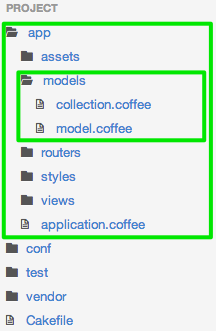
\includegraphics{figures/file-browser.png}
\caption{El visor de archivos: cada vista de directorio contiene más
vistas de archivos de ser necesarias. \label{figure:file-browser}}
\end{figure}

En caso de que el usuario haga click en un archivo, se le pasa la
instancia del modelo al editor de código, el cual indica al modelo que
debe pedir el contenido del archivo al servidor para mostrarlo. El
editor de código es simplemente una librería llamada CodeMirror que
permite al usuario editar el contenido de los archivos. El editor de
código se encarga además de indicarle al modelo del archivo que guarde
su contenido en el backend si el usuario lo solicita.

\textbf{\emph{NO SE SI EXPLICAR MÁS DE LO ANTERIOR}}

Para esta etapa de la construcción, se incluyó además la posibilidad de
ensamblar y ejecutar el proyecto. Para esto, se agregaron métodos en el
modelo de proyectos que hace llamadas al backend para ensamblar y
ejectuar el servidor de pruebas. El evento es manejado por la barra de
navegación, que incluye varios elementos de menú que por esta etapa se
mantuvieron inactivos. A la derecha de la barra de navegación se
encuentra un botón que permite ensamblar y ejecutar el proyecto con un
sólo click, y otros dos que permiten ejecutarlo y ensamblarlo por
separado.

\subsection{Segunda Etapa de Construcción}

La segunda etapa de construccón del proyecto se dedicó principalmente a
la implementación del editor de templates. Dado que esta es la parte más
importante del proyecto se dedicó una etapa completa a ella.

El editor se diseñó de manera que en el centro se tuviera una vista en
vivo de lo que se estaba construyendo, mientras que a la derecha se
listaran todos los componentes disponibles para agregar al template.
Dado que los templates son básicamente HTML, es el navegador el que se
encarga de mostrar cómo se vería finalmente. Por esto, lo que se hizo
fue agregar elementos a la lista de componentes de manera que al
arrastrarlos hacia el centro (el editor), simplemente se agregue su
representación en HTML y el navegador se encargaría de mostrar su
``vista previa''.

Entonces, en la lista de componentes se decidió agregar botones, tablas,
formularios, campos de texto, entre otros, y dentro de ellos (en código,
no visible para el usuario) agregar un fragmento de HTML que se
agregaría al template. Entonces, utilizando jQuery UI\footnote{Definir
  esto!}, cada componente se convierte en un elemento arrastrable. Con
jQuery UI, se necesita convertir elementos en ``arrastrables'' y además,
crear elementos en donde ``soltar'' lo que el usuario está arrastrando.
En este sentido, y, en un primer intento, se convierten todos los
elementos en la vista previa en ``soltables''.

\begin{Shaded}
\begin{Highlighting}[]
\CommentTok{# Con la siguiente llamada, se convierte cada elemento en el editor}
\CommentTok{# de vistas en "soltable".}
\NormalTok{@$}\KeywordTok{(}\StringTok{"*"}\KeywordTok{).}\NormalTok{droppable}\KeywordTok{()}
\end{Highlighting}
\end{Shaded}

Con este primer acercamiento, ya se podía arrastrar y soltar
componentes. El problema es que se podían arrastar componentes como
botones y otras cosas dentro de elementos HTML que no correspondía, como
imágenes, menús, etc. Para esto, se incluyeron ciertas excepciones a la
llamada anterior, como sigue:

\begin{Shaded}
\begin{Highlighting}[]
\CommentTok{# Seleccionar todos los elementos, excepto los que están en la}
\CommentTok{# llamada .not()}
\NormalTok{@$}\KeywordTok{(}\StringTok{"*"}\KeywordTok{).not(}\StringTok{'img, button, input, select, option, optgroup'}\KeywordTok{).}\NormalTok{droppable}\KeywordTok{()}
\end{Highlighting}
\end{Shaded}

Con esto, se simplificó un tanto el arrastrado de componentes, evitando
que algunos quedaran dentro de elementos que no correspondía. Ahora, se
notó que era difícil saber dónde realmente se estaba dejando el
componente que el usuario estaba arrastrando, por lo que se incluyó
retroalimentación visual al momento de arrastar, es decir, cuando el
usuario esté arrastrando el elemento, el elemento en donde ``caería'' el
componente se rodea con un borde amarillo, como muestra la Figura
\ref{asdfaksjdha}. \textbf{\emph{PONER FIGURA!}} Esto se logra usando
propiedades de jQuery UI:

\begin{Shaded}
\begin{Highlighting}[]
\NormalTok{exceptions }\KeywordTok{=} \StringTok{'img, button, input, select, option, optgroup'}
\NormalTok{@$}\KeywordTok{(}\StringTok{"*"}\KeywordTok{).not(}\NormalTok{exceptions}\KeywordTok{).}\NormalTok{droppable}
  \NormalTok{hoverClass}\KeywordTok{:} \StringTok{"hovering"} \CommentTok{# Esto agrega una clase CSS con un borde.}
\end{Highlighting}
\end{Shaded}

La propiedad \texttt{hoverClass} agrega una clase CSS al elemento donde
se estaría arrastrando el componente y la remueve al salir. Con esto se
agrega un borde que facilite al usuario saber dónde caerá el componente.

Se decidió además agregar componentes que sólo sirven si se arrastran
dentro de un formulario. En este punto, el usuario puede arrastrar estos
componentes a cualquier parte, lo que hace de su uso algo complicado.
Para solucionar esto, se implementó un sistema en el cual cada
componente tiene especificado dónde puede ser arrastrado. Por ejemplo,
los botones pueden ser arrastrados a cualquier parte:

\begin{Shaded}
\begin{Highlighting}[]
\KeywordTok{<div}\OtherTok{ class=}\StringTok{"switch-component"}\OtherTok{ data-component-type=}\StringTok{"button"}\KeywordTok{>}
  \KeywordTok{<div}\OtherTok{ class=}\StringTok{"payload"}\KeywordTok{>}
    \KeywordTok{<button}\OtherTok{ type=}\StringTok{"button"}\OtherTok{ class=}\StringTok{"btn btn-primary"}\KeywordTok{>}\NormalTok{Button}\KeywordTok{</button>}
  \KeywordTok{</div>}

  \KeywordTok{<span}\OtherTok{ class=}\StringTok{"name"}\KeywordTok{>}\NormalTok{Button}\KeywordTok{</span>}
\KeywordTok{</div>}
\end{Highlighting}
\end{Shaded}

En cambio, los elementos de un formulario sólo pueden arrastrarse a un
formulario previamente colocado. En el siguiente fragmento se puede
notar la propiedad \texttt{data-component-drop-only} que contiene una
cadena de texto con selectores CSS en dónde puede ser agregado.

\begin{Shaded}
\begin{Highlighting}[]
\KeywordTok{<div}\OtherTok{ class=}\StringTok{"switch-component"}\OtherTok{ data-component-type=}\StringTok{"label-button"} 
\OtherTok{     data-component-drop-only=}\StringTok{"form"}\KeywordTok{>}
  \KeywordTok{<div}\OtherTok{ class=}\StringTok{"payload"}\KeywordTok{>}
    \KeywordTok{<div}\OtherTok{ class=}\StringTok{"control-group"}\KeywordTok{>}
      \KeywordTok{<div}\OtherTok{ class=}\StringTok{"control-label"}\KeywordTok{><label}\OtherTok{ for=}\StringTok{"new_input"}\KeywordTok{>}\NormalTok{Label}\KeywordTok{</label></div>}
      \KeywordTok{<div}\OtherTok{ class=}\StringTok{"controls"}\KeywordTok{>}
        \KeywordTok{<input}\OtherTok{ type=}\StringTok{"text"}\OtherTok{ name=}\StringTok{"new_input"}\OtherTok{ id=}\StringTok{"new_input"}\KeywordTok{>}
      \KeywordTok{</div>}
    \KeywordTok{</div>}
  \KeywordTok{</div>}

  \KeywordTok{<span}\OtherTok{ class=}\StringTok{"name"}\KeywordTok{>}\NormalTok{Form Input}\KeywordTok{</span>}
\KeywordTok{</div>}
\end{Highlighting}
\end{Shaded}

Lo anterior, junto con el siguiente Coffeescript, permite que los
componentes puedan ser arrastrados sólo a ciertos elementos, si es que
lo especifican:

\begin{Shaded}
\begin{Highlighting}[]
\NormalTok{makeDroppable}\KeywordTok{:} \FunctionTok{(only) ->}
  \CommentTok{# Si se especificó only, entonces usarlo, de lo contrario}
  \CommentTok{# permitir cualquier elemento.}
  \KeywordTok{if} \NormalTok{only}
    \NormalTok{only }\KeywordTok{=} \StringTok{"#view_container }\CharTok{#\{}\NormalTok{only}\CharTok{\}}\StringTok{"}
  \KeywordTok{else}
    \NormalTok{only }\KeywordTok{=} \StringTok{"#view_container, #view_container *"}

  \NormalTok{@$}\KeywordTok{(}\NormalTok{only}\KeywordTok{).not(}\NormalTok{exceptions}\KeywordTok{).}\NormalTok{droppable}
    \NormalTok{hoverClass}\KeywordTok{:} \StringTok{"hovering"}
\end{Highlighting}
\end{Shaded}

Hasta ahora, el editor de templates agrega los componentes anexándolos
al final de la posición en la que el usuario las deja. Esto lo
imposibilita de agregar componentes al principio de una lista por
ejemplo. \textbf{\emph{FIGURA EXPLICANDO ESTO?}} Por lo tanto, se agrego
la posibilidad de cambiar ese comportamiento. Al momento de arrastrar un
componente, el usuario puede presionar (y mantener presionada) la tecla
\texttt{SHIFT}, de manera que al dejar un componente, éste se anexe al
principio en vez de al final, permitiendo al usuario agregar cosas al
principio de listas o formularios, por ejemplo.

Por último, para facilitar aún más el arrastrado de componentes, se
agregó una vista previa de cómo quedaría el componente que se está
arrastrando una vez que se suelte. La idea es que al estar arrastrando
un elemento, éste aparece en el editor con una ligera opacidad. Esto se
logró usando algunas llamadas de jQuery UI:

\begin{Shaded}
\begin{Highlighting}[]
\CommentTok{# ...}
\NormalTok{@$}\KeywordTok{(}\NormalTok{only}\KeywordTok{).not(}\NormalTok{exceptions}\KeywordTok{).}\NormalTok{droppable}
  \NormalTok{hoverClass}\KeywordTok{:} \StringTok{"hovering"}
  \NormalTok{greedy}\KeywordTok{:} \OtherTok{yes}
  \NormalTok{drop}\KeywordTok{:} \FunctionTok{(e, u) ->} 
    \NormalTok{self}\KeywordTok{.}\NormalTok{putComponent}\KeywordTok{(}\NormalTok{self}\KeywordTok{,} \NormalTok{$}\KeywordTok{(}\DataTypeTok{this}\KeywordTok{),} \NormalTok{u}\KeywordTok{,} \OtherTok{no}\KeywordTok{)}
  \NormalTok{over}\KeywordTok{:} \FunctionTok{(e, u) ->}
    \NormalTok{self}\KeywordTok{.}\NormalTok{putComponent}\KeywordTok{(}\NormalTok{self}\KeywordTok{,} \NormalTok{$}\KeywordTok{(}\DataTypeTok{this}\KeywordTok{),} \NormalTok{u}\KeywordTok{,} \OtherTok{yes}\KeywordTok{)}
  \NormalTok{out}\KeywordTok{:} \FunctionTok{(e, u) ->} 
    \NormalTok{self}\KeywordTok{.}\NormalTok{removeComponent}\KeywordTok{()}
\end{Highlighting}
\end{Shaded}

Con estas llamadas, al momento de que el usuario esté sobre un elemento
(``over''), literalmente se agrega el componente al editor, para luego
eliminarlo en caso de salirse (``out''), o bien dejarlo definitivamente
al soltarlo (``drop''). \textbf{\emph{FOTOO!!!}}

Por último, el editor de templates también debería permitir al usuario
editar el código directamente, en caso de que no exista algún componente
o bien se necesite agregar cierta lógica más allá de HTML. Para esto, se
utilizó el mismo editor de código que para los archivos normales. Se
agregaron dos pestañas en la parte superior del editor de templates que
permiten cambiar entre el editor visual y el código fuente (ver Figura
\ref{figure:html-editor}).

\begin{figure}[htbp]
\centering
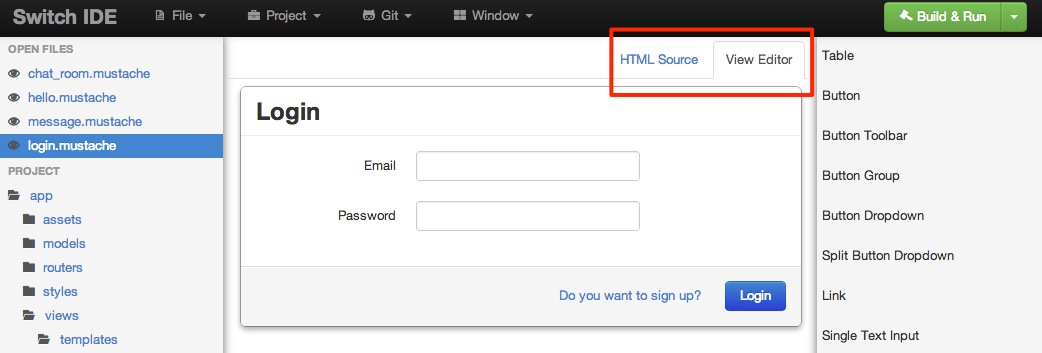
\includegraphics{figures/html-editor.png}
\caption{Estas pestañas permiten al usuario cambiar entre el modo visual
y el editor HTML \label{figure:html-editor}}
\end{figure}

\newpage

\section{Resultados}

\newpage

\section{Conclusiones}

\newpage

\section{Referencias}

{[}1{]} Steve Burbeck, ``Applications Programming in Smalltalk-80(TM):
How to use Model-View-Controller (MVC)'' Disponible:
\href{http://st-www.cs.illinois.edu/users/smarch/st-docs/mvc.html}{http://st-www.cs.illinois.edu/users/smarch/st-docs/mvc.html}.
Última Revisión: 09/07/2012.

{[}2{]} Mike Potel, ``MVP: Model-View-Presenter. The Taligent
Programming Model for C++ and Java'' Disponible:
\href{http://www.wildcrest.com/Potel/Portfolio/mvp.pdf}{http://www.wildcrest.com/Potel/Portfolio/mvp.pdf}.
Última Revisión: 09/07/2012.

{[}3{]} DocumentCloud, ``Backbone'' Disponible:
\href{http://backbonejs.org}{http://backbonejs.org}. Última Revisión:
09/07/2012.

{[}4{]} Backbone, ``Projects and Companies using Backbone'' Disponible:
\href{https://github.com/documentcloud/backbone/wiki/Projects-and-Companies-using-Backbone}{https://github.com/documentcloud/backbone/wiki/Projects-and-Companies-using-Backbone}.
Última Revisión: 09/07/2012.

{[}5{]} Cappuccino Project, ``Cappuccino Framework'' Disponible:
\href{http://www.cappuccino-project.org/}{http://www.cappuccino-project.org/}.
Última Revisión: 09/07/2012.

{[}6{]} Apple Inc., ``Xcode'' Disponible:
\href{https://developer.apple.com/xcode/}{https://developer.apple.com/xcode/}.
Última Revisión: 09/07/2012.

{[}7{]} Sencha Inc., ``Ext JS'' Disponible:
\href{http://www.sencha.com/products/extjs/}{http://www.sencha.com/products/extjs/}.
Última Revisión: 09/07/2012.

{[}8{]} Sencha Inc., ``Ext JS Releases'' Disponible:
\href{http://www.sencha.com/products/releases/}{http://www.sencha.com/products/releases/}.
Última Revisión: 09/07/2012.

{[}9{]} Sencha Inc., ``Buy Ext JS 4 Licenses and Support'' Disponible:
\href{http://www.sencha.com/store/extjs/}{http://www.sencha.com/store/extjs/}.
Última Revisión: 09/07/2012.

{[}10{]} Sencha Inc., ``Sencha Architect'' Disponible:
\href{http://www.sencha.com/products/architect/}{http://www.sencha.com/products/architect/}.
Última Revisión: 09/07/2012.

{[}11{]} Sencha Inc., ``Buy Sencha Architect'' Disponible:
\href{http://www.sencha.com/store/architect/}{http://www.sencha.com/store/architect/}.
Última Revisión: 09/07/2012.

{[}12{]} Divshot, ``Divshot'' Disponible:
\href{http://www.divshot.com}{http://www.divshot.com}. Última Revisión:
09/07/2012.

{[}13{]} Twitter, ``Twitter Bootstrap'' Disponible:
\href{http://getbootstrap.com}{http://getbootstrap.com}. Última
Revisión: 09/07/2012.

{[}14{]} Ian Hickson (editor), ``HTML5 Specification'' Disponible:
\href{http://www.w3.org/TR/2011/WD-html5-20110525/}{http://www.w3.org/TR/2011/WD-html5-20110525/}.
Última Revisión: 09/07/2012.

{[}15{]} eXo Platform SAS, ``eXo Cloud IDE'' Disponible:
\href{http://cloud-ide.com}{http://cloud-ide.com}. Última Revisión:
09/07/2012.

{[}16{]} Git Project, ``Git'' Disponible:
\href{http://git-scm.com}{http://git-scm.com}. Última Revisión:
09/07/2012.

{[}17{]} VMware Inc., ``Wavemaker'' Disponible:
\href{http://wavemaker.com}{http://wavemaker.com}. Última Revisión:
09/07/2012.

{[}18{]} Zoho Corp., ``Zoho Creator'' Disponible:
\href{http://www.zoho.com/creator/}{http://www.zoho.com/creator/}.
Última Revisión: 09/07/2012.

\end{document}
